\documentclass[12pt]{article}

\usepackage{template_wete}
\usepackage{ifthen}

\usepackage{graphicx,url}
\usepackage{multirow} %% essencial %% para uso de tabelas
\usepackage{supertabular} %% essencial %% para uso de tabelas
\usepackage{tabularx} %% essencial %% para uso de tabelas
\usepackage{longtable}
\usepackage{gensymb}
\usepackage{color}
\usepackage{fancyhdr}

\usepackage[brazil, english]{babel}
%\usepackage[latin1]{inputenc}
\usepackage[utf8]{inputenc} %% essencial
\usepackage[T1]{fontenc}

\fancypagestyle{plain}{%
\fancyfoot[LE, RO]{Apurba Paul}
\fancyfoot[LO, RE]{Using fancyhdr}}

%------------------------------------------------------------------------------------------ CABEÇALHOS
\sloppy
\title{Template de Artigo no Word para o 10º Workshop em Engenharia e Tecnologia Espaciais}

\author{FERRARI, N.~\inst{1}, SENNA, A.~\inst{2}}

\address{
	Instituto Nacional de Pesquisas Espaciais, São José dos Campos, SP, Brasil \\
	Aluno de Mestrado do curso de Ciência e Tecnologia de Materiais e Sensores - CMS.
\nextinstitute
	Instituto Tecnológico da Aeronáutica, São José dos Campos, SP, Brasil
\email{autor@inst.br}
}

%\pagestyle{fancy}
\renewcommand{\headrulewidth}{0pt}
\renewcommand{\footrulewidth}{0pt}
\fancyhead{}
\fancyfoot{}

\fancyhead[C]{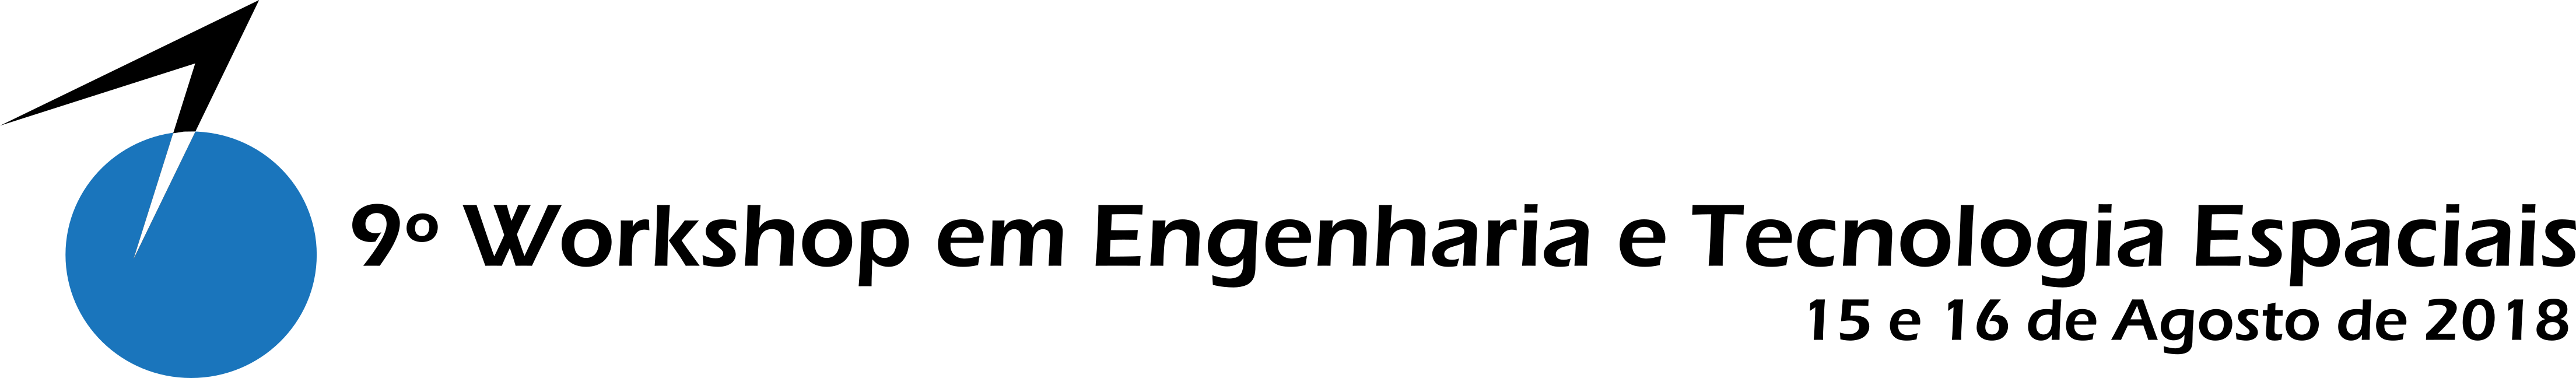
\includegraphics[width=13cm]{logo.png}}
\vspace{3.7cm}
%\fancyhead[R]{São José dos Campos/SP - 07, 08 e 09 de agosto de 2019}

%------------------------------------------------------------------------------------------ CABEÇALHOS

%------------------------------------------------------------------------------------------ CORPO DO TEXTO
\begin{document}

\maketitle

\begin{resumo}
	Apresentação concisa do trabalho, com descrição de suas principais características, principais objetivos, metodologia utilizada e os resultados alcançados. Deve conter entre 50 e 150 palavras, formato justificado; fonte Times tamanho 12; espaço simples.
\end{resumo}
\hrulefill

\begin{flushleft}
	\textbf{Palavras-chave:} De 3 a 5 palavras, iniciadas com letra maiúscula e separadas por ponto e vírgula.
\end{flushleft}

\section{Introdução}

Tem por finalidade apresentar o estado da arte do problema estudado e mostrar um panorama geral sobre o assunto e tema abordado. Deve ser breve e justificar o problema estudado de forma clara, utilizando-se revisão de literatura. O último parágrafo deve conter os objetivos do trabalho realizado.

\section{Metodologia} \label{sec:met}

A seção Metodologia deverá ser concisa e suficientemente clara, para fácil compreensão dos procedimentos utilizados, contendo as referências da metodologia de estudo, o tipo de análise, bem como o tratamento dos dados.

\section{Resultados e Discussão}

Na seção Resultados e Discussão é apresentado o resultado, o que corresponde ao desenvolvimento do trabalho. Os resultados da investigação devem ser apresentados de forma clara, atendendo às características do tipo de dados obtidos.

É nesse item que os dados da pesquisa são interpretados, criticados e comparados com os já existentes sobre o assunto na literatura citada; são discutidas suas possíveis implicações, significados e razões para concordância ou discordância com os autores. A discussão deve fornecer elementos para a conclusão. É o mais livre dos itens e o que mais evidencia a vivência do pesquisador. Se apropriado, podem ser inseridas tabelas (Tabela~\ref{tab:exemploTab1}) e figuras (Figura~\ref{fig:exemploFig1}) das análises feitas.


\begin{longtable}{l l l}
	\caption{Exemplo de Tabela. \textcolor[rgb]{1,0,0}{[Fonte: se aplicável]}}         \\
	\hline
	\textbf{Cidade} & \textbf{Temperatura (\celsius)} & \textbf{Umidade Relativa (\%)} \\
	\hline
	\endfirsthead
	\multicolumn{3}{c}%
	{\tablename\ \thetable\ -- \textit{Continuado da página anterior.}}                \\
	\hline
	\textbf{Cidade} & \textbf{Temperatura (\celsius)} & \textbf{Umidade Relativa (\%)} \\
	\hline
	\endhead
	\hline \multicolumn{3}{r}{\textit{Continua da próxima página.}}                    \\
	\endfoot
	\hline
	\endlastfoot

	Taubaté         & 26                              & 43                             \\
	Ilhéus          & 34                              & 85

	\label{tab:exemploTab1}
\end{longtable}


\begin{figure}[ht]
	\centering
	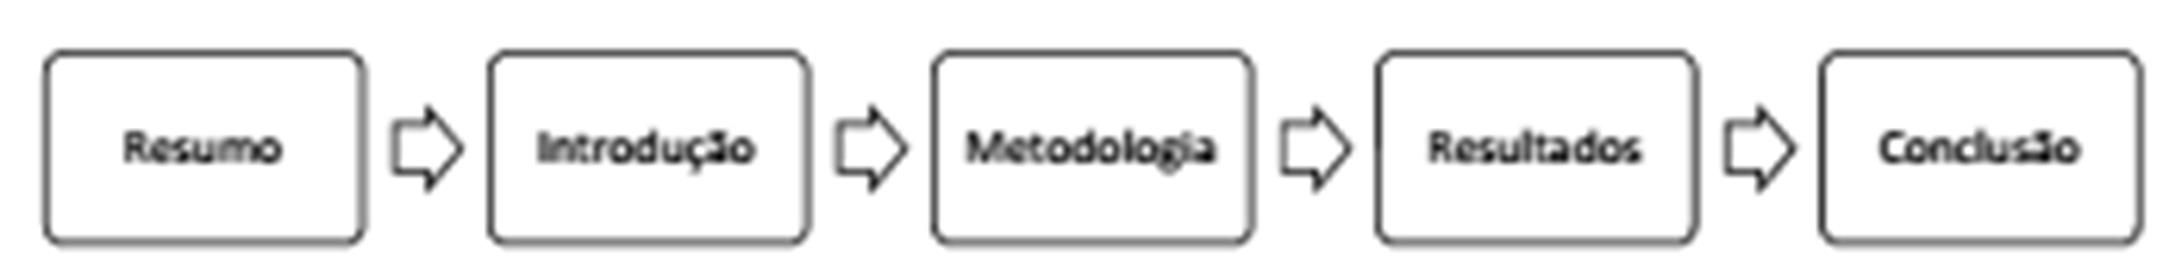
\includegraphics[width=\textwidth]{figura.jpg}
	\caption{Exemplo de figura. \textcolor[rgb]{1,0,0}{[Fonte: se aplicável]} }
	\label{fig:exemploFig1}
\end{figure}

\section{Conclusão}
Constitui o fecho do trabalho e deve ser breve e fundamentada nos resultados obtidos. Deve retornar ao objetivo, inicialmente proposto na seção Introdução, para analisar o quanto foi ou não alcançado.

As referências devem conter apenas as bibliografias citadas como: \cite{knuth:84}, \cite{boulic:91} e \cite{smith:99}.

\begin{flushleft}
	\emph{\textbf{Agradecimentos:} Item destinado a informar agências financiadoras, instituições apoiadoras e colaboradores. \textcolor[rgb]{1,0,0}{(OPCIONAL)}}
\end{flushleft}

%------------------------------------------------------------------------------------------ CHAMA AS REFERÊNCIAS
\bibliographystyle{ref_wete}
\bibliography{referencias}

%------------------------------------------------------------------------------------------ RETIRAR DA VERSÃO FINAL:
\textcolor[rgb]{1,0,0}{
	IMPORTANTE:
	\begin{itemize}
		\item Número de páginas: O trabalho deve conter no \textbf{MÍNIMO 4} e no \textbf{MÁXIMO 8} páginas;
		\item Autor para correspondência: Deve ser apresentado apenas 1 e-mail para correspondência;
		\item Citações: As citações devem ser feita por: [SOBRENOME DOS AUTORES ANO];
		\item Referência: A seção Referência deve ser apresentada em ordem alfabética;
		\item Identificação dos Autores:
		\item Na descrição o autor deverá informar a situação acadêmica atual (ex: aluno de mestrado/doutorado, mestre ou doutor) e a área de concentração da ETE a qual está vinculado. Ver exemplo abaixo.;
		\item Agradecimentos: Se o primeiro autor for bolsista (CAPES, CNPq, FAPESP), o mesmo deverá citar a agência financiadora no item Agradecimentos.
	\end{itemize}
	%\small{
	Identificação:\\
	Para alunos do INPE:\\
	Nome completo\\
	Situação do aluno (Mestrando/Doutorando)  na PG-ETE e a área de concentração. Exemplo: Mestrando em Engenharia e Gerenciamento de Sistemas Espaciais\\
	Instituto Nacional de Pesquisas Espaciais\\
	Para orientadores: (INPE)\\
	Nome completo\\
	Divisão / Departamento que atua no INPE\\
	Instituto Nacional de Pesquisas Espaciais\\
	Para Orientadores (externos ao INPE):\\
	Nome completo\\
	Departamento que atua\\
	Instituição de Ensino / Empresa\\
	Para alunos de Iniciação Científica:\\
	Nome completo\\
	Iniciação Científica na Divisão xxxxx\\
	Instituto Nacional de Pesquisas Espaciais\\
	Para alunos de Graduação externos ao INPE:\\
	Nome completo\\
	Nome do curso\\
	Instituição de Ensino\\
	Para os orientadores dos alunos de Graduação externos ao INPE:\\
	Nome completo\\
	Departamento na Instituição de Ensino\\
	Instituição de Ensino\\
	%}
}
\end{document}
%------------------------------------------------------------------------------------------ CORPO DO TEXTO
